\renewcommand*{\arraystretch}{1.5}
\begin{tabularx}{15cm}{|p{2.1cm}@{\hskip 1ex}|@{\hskip 1ex}X|}
	\hline
	number      & 22                                                          \\ \hline
	title       & International dialog                                                           \\ \hline
	\multicolumn{2}{|c|}{ 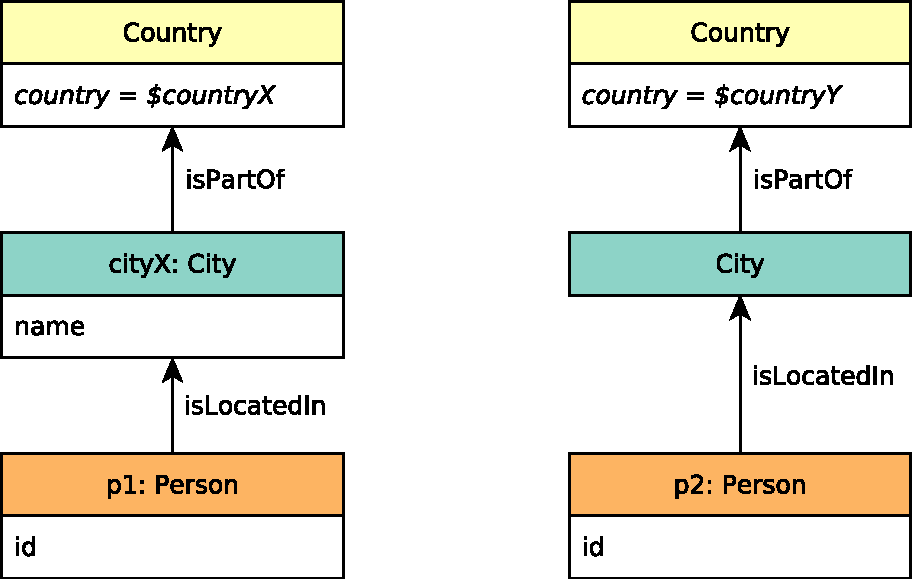
\includegraphics[scale=\patternscale,margin=0cm .2cm]{patterns/q22}} \\ \hline
	description & Consider all pairs of people \texttt{(p1,\ p2)} such that one is located
in a city of Country \texttt{countryX} and the other is located in a
city of Country \texttt{countryY}.

For each city of Country \texttt{countryX}, return the highest scoring
pair.

The score of a pair is defined as the sum of the scores of the following
kinds of interaction:

\begin{itemize}
\tightlist
\item
  \texttt{p1} has created a reply Comment to at least one Comment or
  Post by \texttt{p2}: \texttt{Score\ =\ 4}
\item
  \texttt{p1} has created at least one Post or Comment that \texttt{p2}
  has created a reply Comment to: \texttt{Score\ =\ 1}
\item
  \texttt{p1} and \texttt{p2} Know each other: \texttt{Score\ =\ 15}
\item
  \texttt{p1} liked at least one Post or Comment by \texttt{p2}:
  \texttt{Score\ =\ 10}
\item
  \texttt{p1} has created at least one Post or Comment that was liked by
  \texttt{p2}: \texttt{Score\ =\ 1}
\end{itemize}

I.e., the maximum score a pair can obtain is:
\texttt{4\ +\ 1\ +\ 15\ +\ 10\ +\ 1\ =\ 31}
 \\ \hline
	
	parameters  &
	\multicolumn{1}{>{\raggedright}X|}{
		\variable{countryX}{String} \\
		\variable{countryY}{String} 
		}\\ \hline
	result      &
	\multicolumn{1}{>{\raggedright}X|}{
		\variable{p1.id}{64bitInteger}\\
		\variable{p2.id}{64bitInteger}\\
		\variable{cityX.name}{String}\\
		\variable{score}{32bitInteger}
		}\\ \hline
	sort        &
	\multicolumn{1}{>{\raggedright}X|}{
		\sortentry{score}{\desc}\\
		\sortentry{p1.id}{\asc}\\
		\sortentry{p2.id}{\asc}
		}\\ \hline
	choke points        &
	\multicolumn{1}{>{\raggedright}X|}{
		\chokepoint{1.4}, 
		\chokepoint{1.6}, 
		\chokepoint{2.1}, 
		\chokepoint{3.1}, 
		\chokepoint{3.3}, 
		\chokepoint{5.1}, 
		\chokepoint{5.2}, 
		\chokepoint{5.3}
		}\\ \hline
\end{tabularx}
\clearpage
